\documentclass{article}
\usepackage{polski}
\usepackage[utf8]{inputenc}
\title{Transformacja Fouriera}
\author{Mateusz Rutkiewicz}
\usepackage[rightcaption]{sidecap}
\usepackage{graphicx} % \scalebox
\usepackage{pgfplots}
\pgfplotsset{compat=1.15}
\begin{document}
\maketitle

\Large
\section{Wprowadzenie}

\subsection{Wzór} 

Transformacja Fouriera opiera się o zsumowaniu iloczynu dwóch funkcji (sygnałów): sygnału wejściowego $x(n)$ oraz funkcji $f(n) = e^{-\frac{2\pi i}{N}nk}$.

\begin{equation}
    X_k = \sum_{n=0}^{N-1} x_n e^{-\frac{2\pi i}{N}nk}
\end{equation}{}

\subsection{$e^{ix}$ (liczna Eulera podniesiona do liczby urojonej)} 

Sens podnoszenia do potęgi liczby urojonej uzyskuje się z szeregu potęgowego (szeregu Taylora). Dla $e^x$:

\begin{equation}
    e^x = \sum_{n=0}^\infty \frac{x^n}{n!}
\end{equation}

\begin{equation}
    e^{ix} = \sum_{n=0}^\infty \frac{(ix)^n}{n!}
\end{equation}

\begin{equation}
    e^{ix} = \frac{(ix)^0}{0!} + \frac{(ix)^1}{1!} + \frac{(ix)^2}{2!} + \frac{(ix)^3}{3!} + \frac{(ix)^4}{4!} + \frac{(ix)^5}{5!} + ...
\end{equation}

\begin{equation}
    e^{ix} = \frac{x^0}{0!} + \frac{ix^1}{1!} - \frac{x^2}{2!} - \frac{ix^3}{3!} + \frac{x^4}{4!} + \frac{ix^5}{5!} + ...
\end{equation}

\begin{equation}
    e^{ix} = 
    \underbrace{(1 -\frac{x^2}{2!} + \frac{x^4}{4!} + ...)}_{cos(x)} +
    \underbrace{i(x - \frac{x^3}{3!}  + \frac{x^5}{5!} + ...)}_{isin(x)}
\end{equation}

Z szeregu Taylora:

\begin{equation}
    sin(x) = \sum_{x=0}^\infty \frac{(-1)^nx^{2n+1}}{(2n+1)!} = x - \frac{x^3}{3!} + \frac{x^5}{5!} - \frac{x^7}{7!} + ...
\end{equation}

\begin{equation}
    cos(x) = \sum_{x=0}^\infty \frac{(-1)^nx^{2n}}{(2n)!} = 1 - \frac{x^2}{2!} + \frac{x^4}{4!} - \frac{x^6}{6!} + ...
\end{equation}

Oznacza to, że zapis $|z|e^{i\phi}$ odpowiada reprezentacji trygonometrycznej liczby zespolonej $|z|(cos(\phi) + isin(\phi))$, gdzie $|z|$ jest modułem liczby zespolonej (odległością od punktu $(0 + i0)$), a $\phi$ kątem odchylenia od osi rzeczywistej.

Samo $e^{ix}$ pozwala jedynie na zapisanie wartości, które leżą na okręgu o środku $S=0+i0$ i promieniu $r=1$. Szczególną równością jest tutaj tożsamość Eulera:

\begin{equation}
    e^{i\pi}=-1
\end{equation}

Warto też zaznaczyć, że funkcja $f(x) = e^{ix}$ jest okresowa. Od $e^{2*i\pi}$ wartości się powtarzają.

\begin{equation}
    e^{2*i\pi}=e^0=1
\end{equation}

\begin{SCfigure}[0.5][ht]
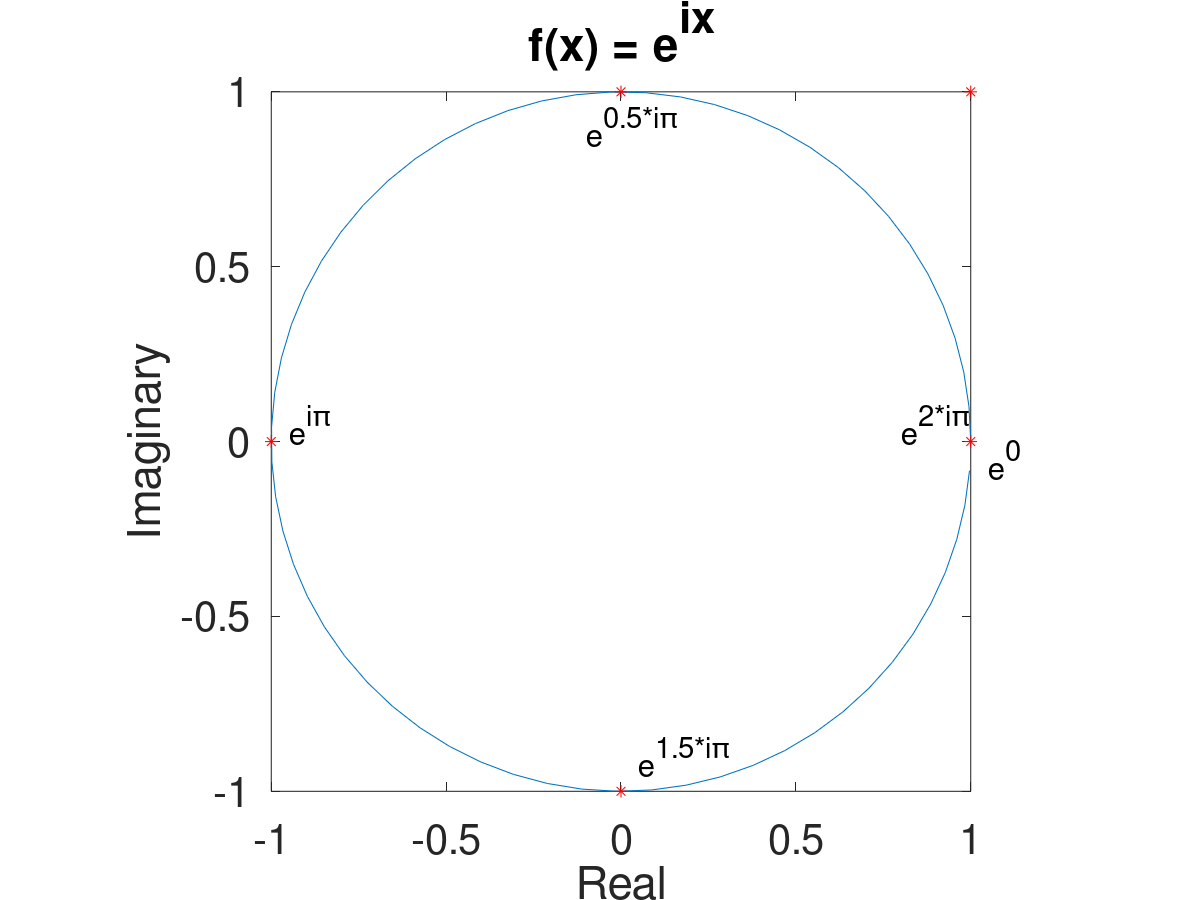
\includegraphics[width=1\textwidth]{euler.png}
\caption{}
\end{SCfigure}

\section{Interpretacja Transformacji Fouriera} 
\subsection{Mnożenie}

Transformacja Fouriera korzysta z wyrażenia:

\begin{equation}
e^{-\frac{2\pi i}{N}nk}
\end{equation}

$-2\pi i$ to kąt pełny razy część urojona.

$\frac{n}{N}$ to wyrażenie dające rosnąco wartości $[0, 1)$, dla n rosnącego od $0$ do $N-1$

W takim wypadku samo wyrażenie:

\begin{equation}
    X_n = x_n e^{-\frac{2\pi i}{N}n}, n = 0, 1, 2, ..., N-1
\end{equation}

pozwala przemnożyć sygnał przez okrąg z wykresu wyżej.

Na przykład, dla $sin(0.1x_n)$, dla x od $0$ do $2\pi$  uzyskujemy taki wykres:

\begin{SCfigure}[0.5][ht]
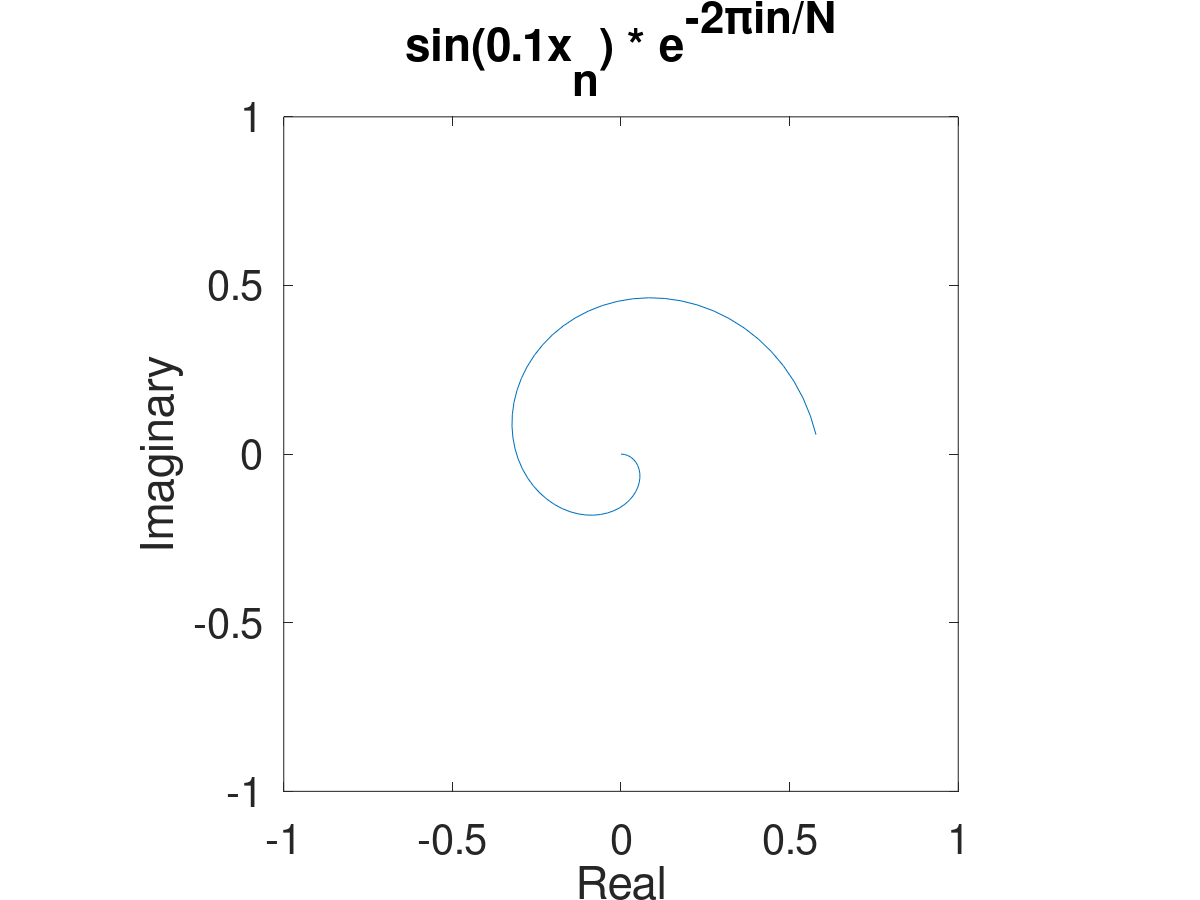
\includegraphics[width=1\textwidth]{fourier.png}
\caption{}
\end{SCfigure}

To jest prosty przykład, sygnał który będę analizował ma taką postać:

\begin{equation}
    \frac{1}{2}(sin(2x) + sin(5x))
\end{equation}

i daje taki wykres:

\begin{SCfigure}[0.5][ht]
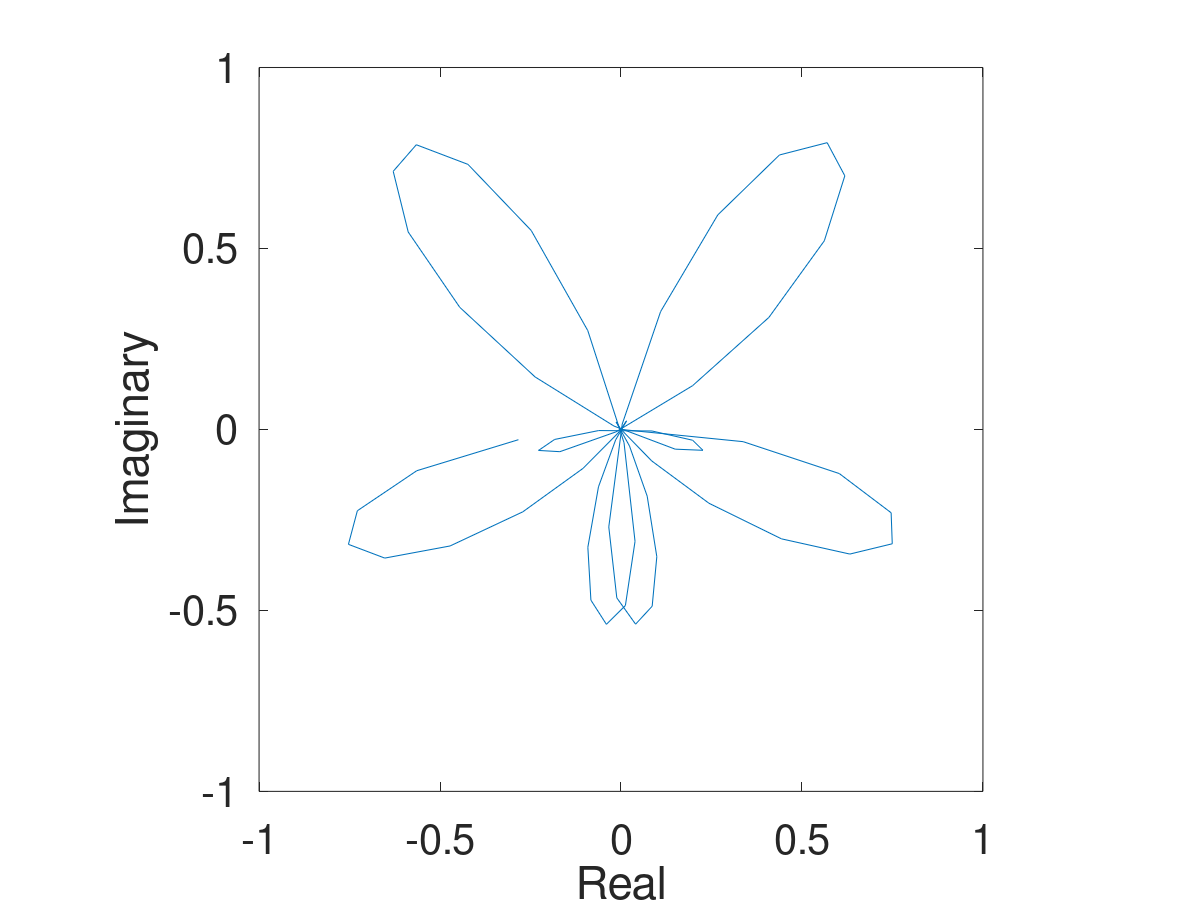
\includegraphics[width=1\textwidth]{fourier2.png}
\caption{}
\end{SCfigure}

W samej formule brakuje jedynie $k$, które służy jako częstotliwość (sygnał z rysunku Fourier2 ma częstotliwości $k=2$ oraz $k=5$) oraz sumowania.

\subsection{Sumowanie}
Sumowanie w tym wypadku zastępuje całkowanie z niedyskretnej Transformacji Fouriera. Cechą całki w Transformacji Fouriera jest to, że daje wartości zbliżone do zera, jeżeli w sygnale nie ma częstotliwości $k$, natomiast gdy $k$ zbliża się do występującej w sygnale częstotliwości, wynik Transformacji Fouriera będzie się oddalał od zera. Czerwone punkty na wykresach to wyniki Transformacji Fouriera. Dla poprzedniego sygnału:

\begin{SCfigure}[0.2][htbp]
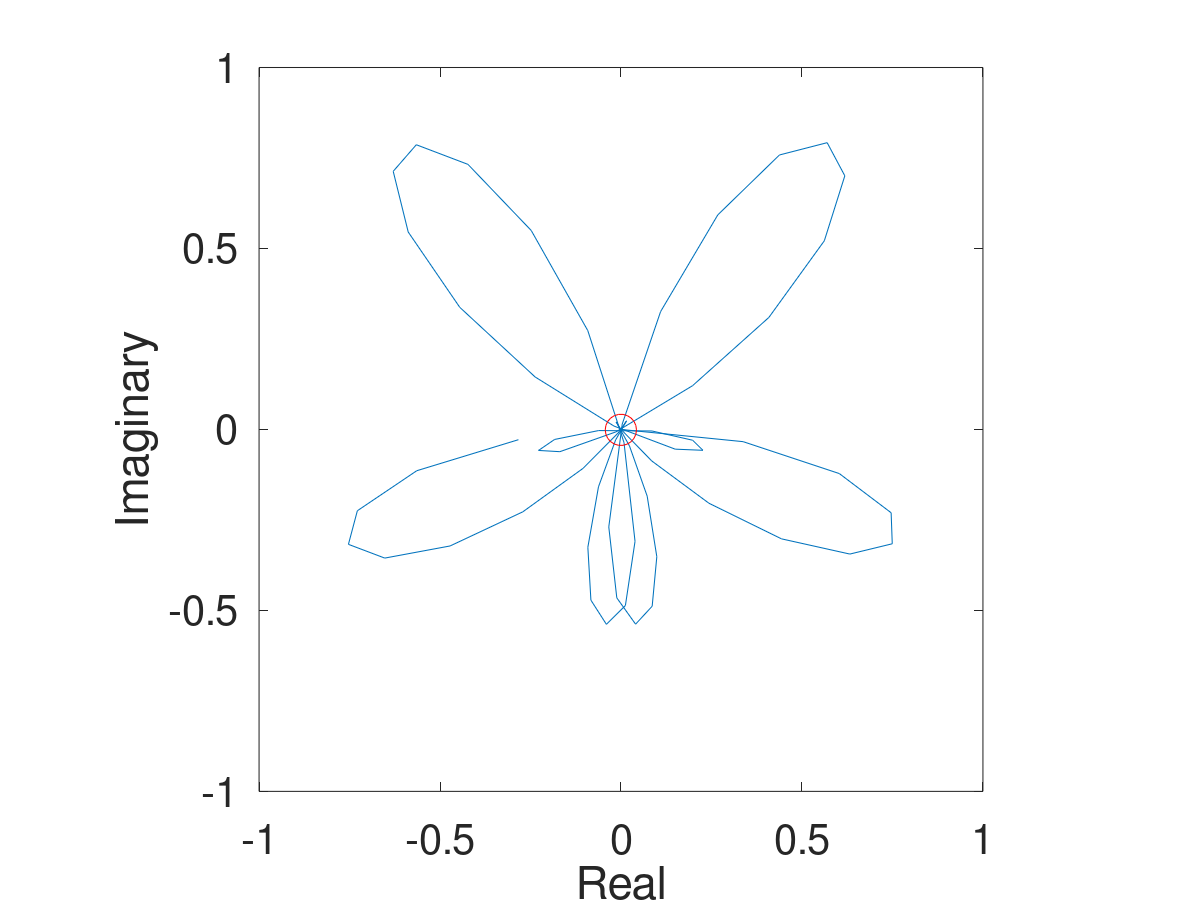
\includegraphics[width=1\linewidth]{fourier3.png}
\caption{k=1}
\end{SCfigure}

\begin{SCfigure}[0.2][htbp]
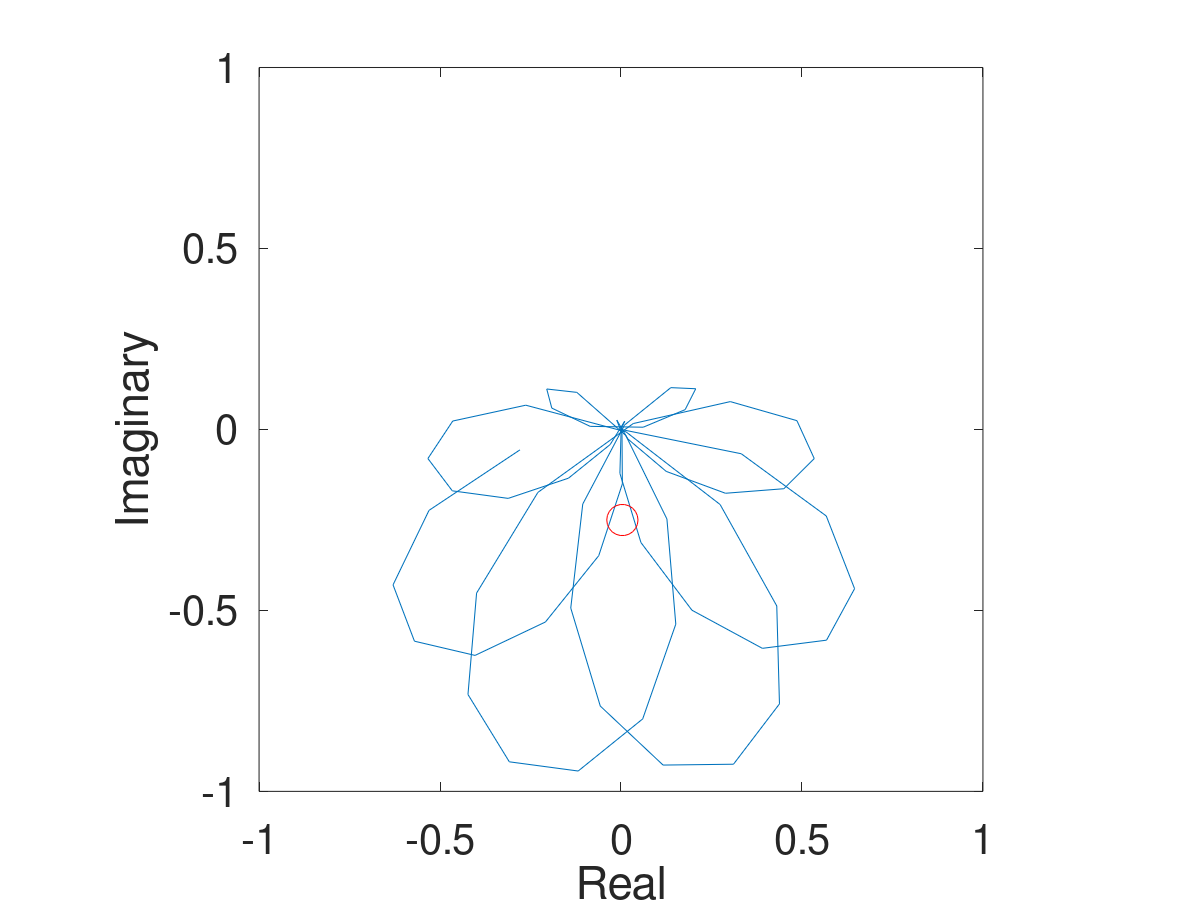
\includegraphics[width=1\linewidth]{fourier4.png}
\caption{k=2}
\end{SCfigure}

\begin{SCfigure}[0.2][htbp]
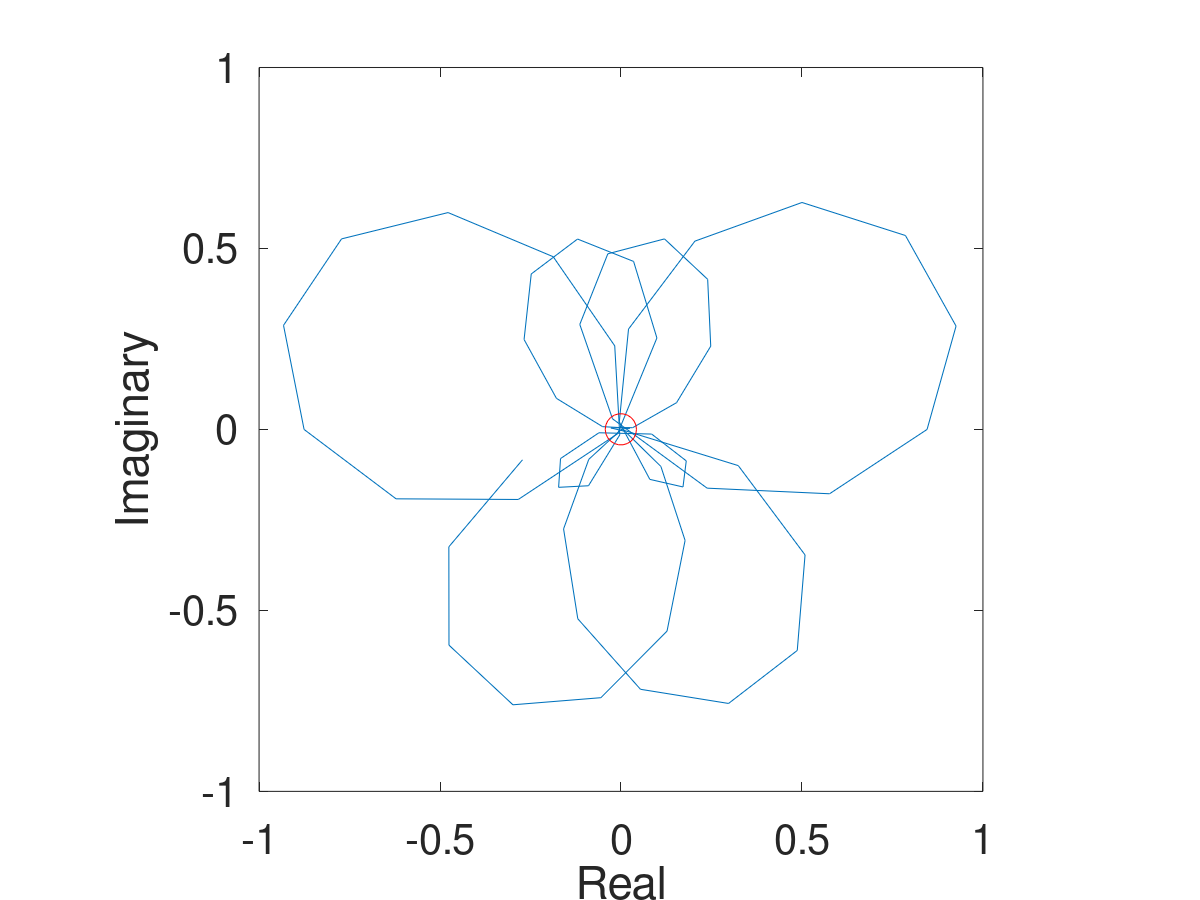
\includegraphics[width=1\linewidth]{fourier5.png}
\caption{k=3}
\end{SCfigure}

\begin{SCfigure}[0.2][htbp]
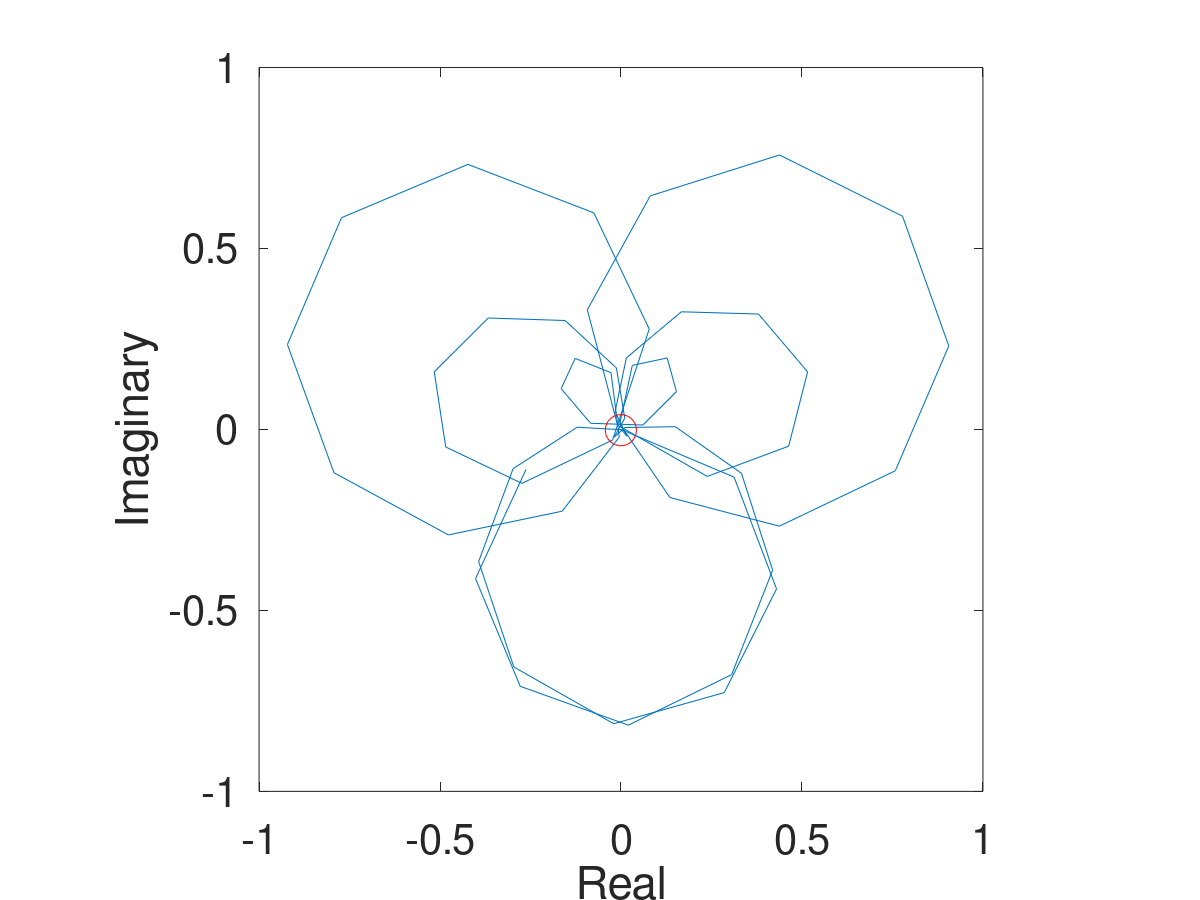
\includegraphics[width=1\linewidth]{fourier6.png}
\caption{k=4}
\end{SCfigure}

\begin{SCfigure}[0.2][htbp]
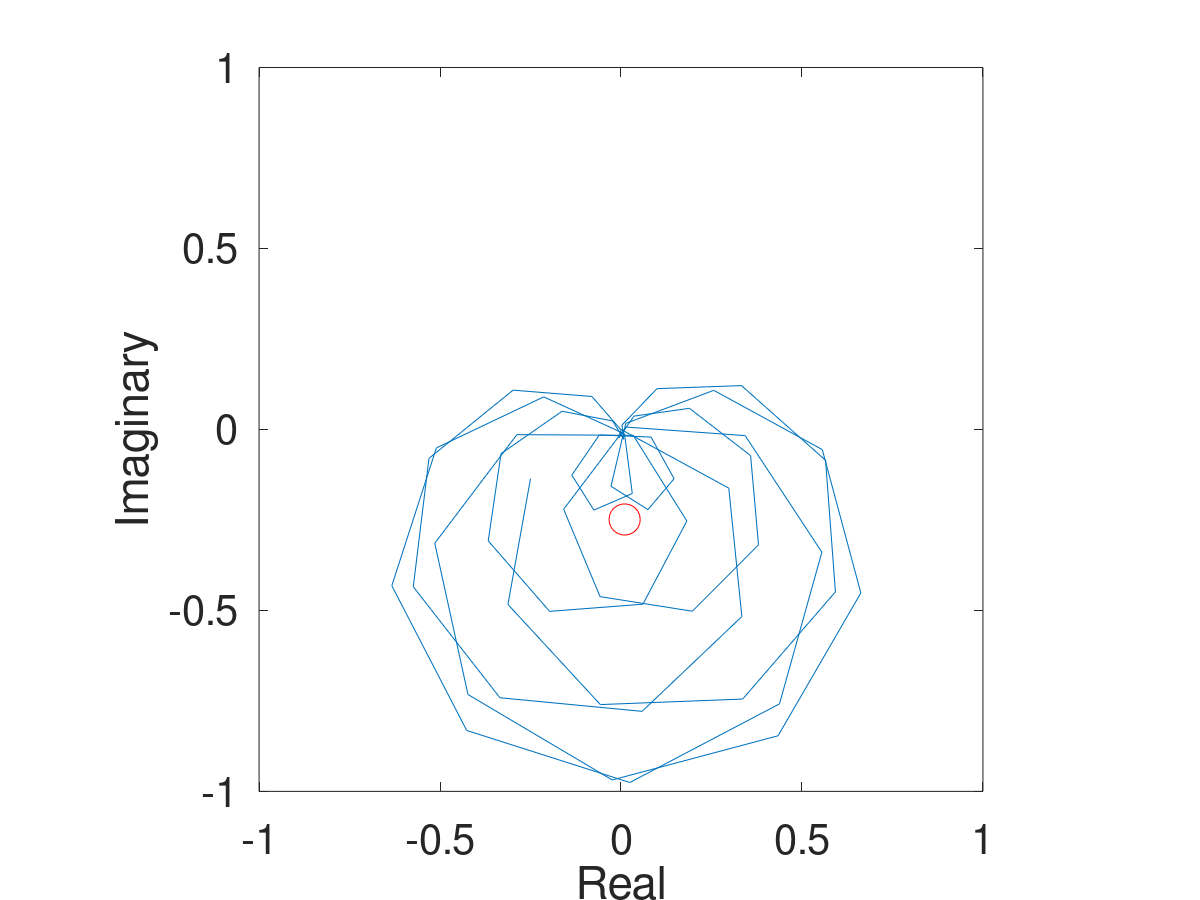
\includegraphics[width=1\linewidth]{fourier7.png}
\caption{k=5}
\end{SCfigure}

\begin{SCfigure}[0.2][htbp]
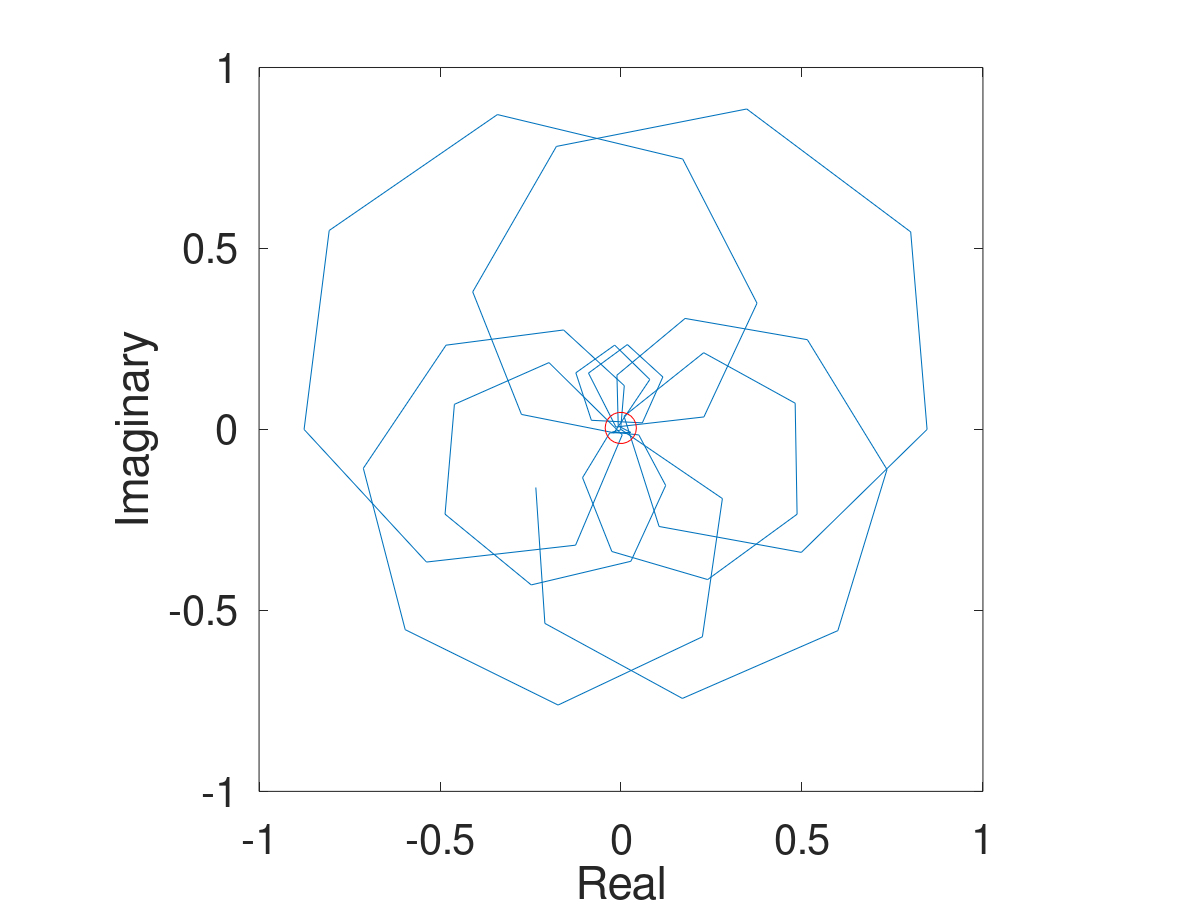
\includegraphics[width=1\linewidth]{fourier8.png}
\caption{k=6}
\end{SCfigure}

Notatka: Wyniki Dyskretnej Transformacji Fouriera został przeskalowany przez ilość próbek sygnału $\frac{1}{N}$ tak, by wartości zwracane przez nią mieściły się na wykresie. W ten sposób są w przybliżeniu wartościami uzyskiwanymi przy Niedyskretnej Transformacji Fouriera.

\newpage

Jak widać, dla danych częstotliwości sygnał oddala się od zera.

Po wykonaniu pełnej Transformacji Fouriera otrzymujemy taki wynik (na wykresie przedstawione są jedynie wartości bezwzględne liczb zespolonych):

\begin{SCfigure}[0.5][htbp]
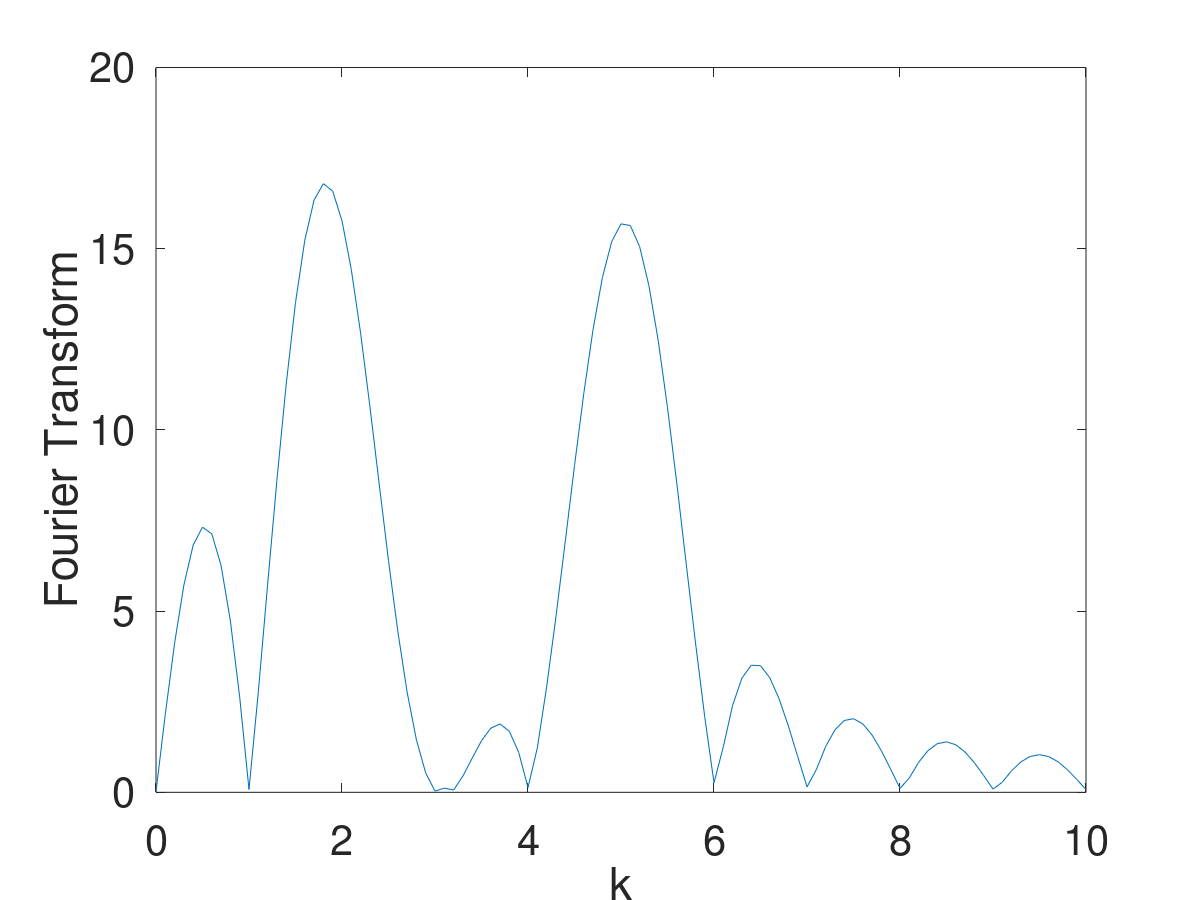
\includegraphics[width=1\linewidth]{fourier9.png}
\caption{}
\end{SCfigure}

\end{document}
